So far in this book, we have concentrated on message-passing concurrency,
together with barrier synchronisations to synchronise threads.  In the next
few chapters, we will look at other concurrency primitives.  These typically
operate at a lower level of abstraction.  They are often built in to the
hardware, the operating system, or the programming language implementation.
This tends to make them more efficient.  However, they tend to be harder to
use, and less intuitive, than message passing, which is why we started this
book with the latter.

In this chapter we will see how to use explicit locks.  An SCL lock can be
created as follows:
%
\begin{scala}
  val lock = new Lock
\end{scala}

A lock has two principle operations:
%
\begin{itemize}
\item |acquire()|: wait until no other thread holds the lock, and then acquire
  it;

\item |release()|: release the lock.
\end{itemize}
%
At most one thread can hold the lock at a time.  Hence this gives us a way to
enforce mutual exclusion, for example, to avoid races.

We will see other uses of locks in the next chapter. 
%
Most other programming languages provide an implementation of locks with a
similar interface.

Figure~\ref{fig:counter-lock0} gives a simple example, based on the counter
example from Chapter~\ref{chap:intro}.  A lock is used to protect the counter
variable~|c|.  Each operation accesses~|c| only when it is holding the lock.
This means that it accesses~|c| under mutual exclusion, so two different
operations cannot interfere.

%%%%%

\begin{figure}
\begin{scala}
class Counter0{
  /** The value of the counter. */
  private var c = 0

  /** Lock used to protect £c£. */
  private val lock = new Lock

  /** Increment the counter. */
  def inc() = { lock.acquire(); c += 1; lock.release() }

  /** Decrement the counter. */
  def dec() = { lock.acquire(); c -= 1; lock.release() }

  /** Get the value of the counter. */
  def get: Int = { lock.acquire(); val result = c; lock.release(); result }
}
\end{scala}
\caption{A simple implementation of a counter, using a lock.}
\label{fig:counter-lock0}
\end{figure}

%%%%%

Note that the |get| operation copies the value of~|c| into a local
variable~|result| before releasing the lock and returning~|result|.  There are
a number of variants that do \emph{not} work, including the following.
\begin{itemize}
\item \SCALA{def get1: Int = \{ lock.acquire(); c; lock.release() \}}.  This
  does not work, because it doesn't return~|c|.  It returns the value of the
  final command in the sequence, namely |lock.release()|; this has type
  |Unit|, so in fact this definition doesn't typecheck.

\item \SCALA{def get2: Int = \{ lock.acquire(); return c; lock.release() \}}.
  This does not work, because it returns as soon as it reaches the |return|
  statement, so it doesn't release the lock!  No subsequent operation will be
  able to proceed.
\end{itemize}

\begin{instruction}
Make sure you understand the code in Figure~\ref{fig:counter-lock0}.
\end{instruction}

%%%%%

The |Lock| class also contains the following helper function, which performs
the computation~|comp| under mutual exclusion.
\begin{scala}
  /** Execute £comp£ under mutual exclusion for this lock. */
  def mutex[A](comp: => A): A = {
    acquire(); try{ comp } finally{ release() }
  } 
\end{scala}
%
(This is defined within the |Lock| class, to here |acquire| and |release| are
operations on the relevant lock object.)

The type ``\SCALA{=> A}'' means that the parameter |comp| is passed \emph{by
  name}.  Most parameters are passed in Scala are passed by value, which means
that they are evaluated \emph{before} the body of the function is executed.
That isn't what we want here, because it would mean that |comp| would be
evaluated before the lock is acquired, negating the intention!  Instead, the
computation |comp| is performed at the point it appears in the definition of
|mutex|, i.e.~after the lock is acquired.

The |finally| clause ensures that the lock is released after |comp| is
complete.  In particular, if |comp| returns a value, that value is calculated
and stored \emph{before} the lock is released: this avoids the necessity to
use a temporary variable discussed earlier.

Figure~\ref{fig:counter-lock} illustrates the use of the |mutex| function.
Every operation is simply wrapped inside an application of |mutex| on the
lock.  This makes it very each to provide mutual exclusion.  

%%%%%

\begin{figure}
\begin{scala}
class Counter extends CounterT{
  /** The value of the counter. */
  private var c = 0

  /** Lock used to protect c. */
  private val lock = new Lock

  /** Increment the counter. */
  def inc() = lock.mutex{ c += 1 }

  /** Decrement the counter. */
  def dec() = lock.mutex{ c -= 1 }

  /** Get the value of the counter. */
  def get: Int = lock.mutex{ c}
}
\end{scala}
\caption{A simple implementation of a counter, using a lock and {\scalashape
    mutex} blocks.}
\label{fig:counter-lock}
\end{figure}


Using |mutex| also means that if some code has several different branches, we
don't need to release the lock explicitly at the end of \emph{every} branch:
with explicit releasing, it is easy to miss a branch in such cases. 

%%%%%%%%%%%%%%%%%%%%%%%%%%%%%%%%%%%%%%%%%%%%%%%%%%%%%%%

%\subsection{Re-entry}

Consider an object that contains the following code
%
\begin{scala}
  private val lock = new Lock
  def f(x: Int) = lock.mutex{ ...; g(y); ... }
  def g(y: Int) = lock.mutex{ ... }
\end{scala}
%
Here the function~|f| calls the function~|g|, and both functions use a |mutex|
block.  That means that if a thread in~|f| gets to the call of~|g|, it already
holds the lock, but has to obtain it again.

The implementation of a |Lock| allows this: if a thread holds the lock, it can
acquire it again.  We say that the lock is \emph{re-entrant}.  Internally, the
implementation records how many times the thread holds the lock: it needs to
release the lock a corresponding number of times before another thread can
acquire it.  In the above example, if a thread in~|f| enters~|g|, it holds the
lock twice; when |g| returns, it holds the lock once; only when |f| returns
can another thread obtain the lock. 

%%%%%%%%%%  \heading{Java Memory Model}

Recall the discussion of memory caches from Chapter~\ref{chap:intro}: when a
thread reads a shared variable, it may read the value from its cache, and so
obtain an out-of-date version; when a thread writes to a shared variable,
initially the write happens only in the thread's cache, so the new value might
not be available to other threads.

Correct use of a |Lock| avoids these problems.  When a thread releases a
|Lock|, it \emph{publishes} the values in the cache, making them available to
other threads.  When a thread aquires a |Lock|, it \emph{subscribes} to all
variables published by other threads on the same |Lock|.  This means that if
all accesses to a variable are protected by a particular |Lock|, as in
Figure~\ref{fig:counter-lock}, then any read of the variable is guaranteed to
see the most-recent value written by another operation.  Further, compiler
optimisations must respect this semantics.  This means that if you are using
|Lock|s correctly to protect against data races, you do not need to worry
about the memory consistency.

%%%%%%%%%%%%%%%%%%%%%%%%%%%%%%%%%%%%%%%%%%%%%%%%%%%%%%%%%%%%

\section{Implementing Concurrent Objects with Locks}

A number of concurrent objects can be implemented using locks.  Remember, the
idea here is that a concurrent object should provide thread-safe operations:
executions of different executions should not interfere.  This can be achieved
by each operation execution locking the object, so as to provide mutual
exclusion.  This strategy is appropriate for \emph{total} operations, where
the operation can return a result in an arbitrary state.  However, it is no
appropriate for partial operations or synchronisation objects, where a thread
may have to wait: this will require an additional mechanism, which we will see
in the next chapter.

Figure~\ref{fig:LockTotalQueue} gives an implementation of a total queue (see
Section~\ref{sec:total-queue}), implemented using a lock.  Each of the main
operation simply performs the operation on the encapsulated |Queue|, while
achieving mutual exclusion using a |Lock|.  (We include the |shutdown|
operation simply to match the |TotalQueue| trait, but it is a no-op in this
case.) 

%%%%%

\begin{figure}
\begin{scala}
class LockTotalQueue[T] extends TotalQueue[T]{
  /** The current state of the queue. */
  private val queue = new Queue[T]

  /** A £Lock£ to protect queue. */
  private val lock = new Lock

  /** Enqueue £x£. */
  def enqueue(x: T) = lock.mutex{ queue.enqueue(x) }

  /** Try to dequeue.  Return £None£ if the queue is empty. */
  def dequeue(): Option[T] = lock.mutex{ 
    if(queue.isEmpty) None else Some(queue.dequeue()) 
  }

  /** Shutdown the queue. */
  def shutdown() = {} // Nothing to do.
}
\end{scala}
\caption{A total queue implemented using a lock.}
\label{fig:LockTotalQueue}
\end{figure}

%%%%%

\begin{instruction}
Study the details of the implementation.
\end{instruction}

%%%%%

As another example, Figure~\ref{fig:BagOfTasksLock} gives an implementation of
the bag-of-tasks object (see Figure~\ref{fig:BoT-interfaces}) from the
trapezium rule example, using a lock.  (Exercise~\ref{ex:summer-monitor} asks
you to implement the other concurrent object from that example.)  Recall that
objects of the |BagOfTasks| trait provide an operation |getTask| that returns
a |Task| (a four-tuple), or the value |null| if there are no further |Task|s
to perform.

%%%%%

\begin{figure}
\begin{scala}
/** The bag of tasks object, using a Lock. */
class BagOfTasksLock(a: Double, b: Double, n: Long, nTasks: Int)
    extends BagOfTasks{ 
  /** The size of each interval. */
  private val delta = (b-a)/n

  /** Number of tasks issued so far. */
  private var i = 0

  /** Lock protecting £i£. */
  private val lock = new Lock

  /** Boundary of the £i£th task.  The number of intervals in tasks £[0..i)£. */
  @inline private def boundary(i: Int) = n*i/nTasks

  /** The £i£th task. */
  @inline private def getTask(i: Int): Task = {
    val b1 = boundary(i); val b2 = boundary(i+1)
    val taskSize = b2-b1; val left = a+b1*delta; val right = a+b2*delta
    (left, right, taskSize.toInt, delta)
  }

  /** Get a task, or £null£ if there are no more tasks. */
  def getTask(): Task = {
    var myI = -1
    lock.mutex{ myI = i; i += 1} // Get and increment £i£.
    if(myI < nTasks) getTask(myI) else null
  }
}
\end{scala}
\caption{The bag-of-tasks object implemented using a lock.}
\label{fig:BagOfTasksLock}
\end{figure}

%%%%%

It is tempting to use a |mutex| block for the whole of the |getTask|
operation.  However, this operation creates a bottleneck for the application.
It is more efficient to make the mutual exclusion operation as small as
possible, to minimise the bottleneck.  To this end, the object maintains a
variable~|i| representing the number of tasks issued so far.  A short |mutex|
block copies the value of~|i| into a thread-local variable, and increments~|i|
ready for the next thread.  Straightforward code then calculates the required
|Task| from the thread-local copy.  This means that several threads can be
performing this calculation concurrently: a thread needs to wait only for the,
hopefully short, period when another thread holds the lock.

%%%%%

Figure~\ref{fig:bag-of-tasks-experiment-monitors}
%and~\ref{fig:bag-of-tasks-experiment-monitors-2} 
gives experimental results based on this implementation.  The two graphs are
directly comparable with Figures~\ref{fig:bag-of-tasks-experiment}
and~\ref{fig:bag-of-tasks-experiment-2}, respectively.

\begin{figure}
\begin{center}
\begin{tikzpicture}
\begin{semilogxaxis}[
%  title = Timing experiment on the numerical integration example,
  ylabel = Time (ms),
%  legend pos = north east,
  legend style={at={(0.70,0.98)}},
  height = 0.4\textheight,
  width = 0.85\textwidth,
  scaled ticks = false,
%  title = Experiment on the numerical integration bag-of-tasks example.,
  xlabel = Number of workers,
  log basis x=2,
  ymin = 500,
  ymax = 5000
]
\addplot+[error bars/.cd, y dir=both,y explicit] coordinates {
  (1,5182.6512094) +- (0,26.098472725675258)
  (2,2855.4097185) +- (0,27.79352075670627)
  (4,1644.7399939411764) +- (0,16.347855934496295)
  (8,1497.77329874) +- (0,20.217084622680833)
  (16,2062.5562124000003) +- (0,23.569186907602198)
  (32,3029.0620465) +- (0,30.207086355269553)
  (64,4734.277534214286) +- (0,46.19852418281014)
};
\addlegendentry{$\sm n = 2^{18}$; $2^{9}$ tasks}
\addplot+[error bars/.cd, y dir=both,y explicit] coordinates {
  (1,4923.3609956) +- (0,28.971252450123718)
  (2,2640.8397855999997) +- (0,25.77840063706191)
  (4,1449.4778961714287) +- (0,14.37115217239129)
  (8,1047.5968940599998) +- (0,23.012316305531392)
  (16,1192.5654679000002) +- (0,24.131222447999765)
  (32,1392.86203508) +- (0,25.748348780536308)
  (64,2026.57816696) +- (0,22.753597135746322)
};
\addlegendentry{$\sm n = 2^{20}$; $2^{10}$ tasks}
\addplot+[error bars/.cd, y dir=both,y explicit] coordinates {
  (1,4863.096237199999) +- (0,31.29992991506052)
  (2,2510.5514174444447) +- (0,22.85025865889476)
  (4,1373.969332097561) +- (0,13.631653403779632)
  (8,868.5689277) +- (0,16.386592853918252)
  (16,919.92892792) +- (0,21.54772596772679)
  (32,1012.21671764) +- (0,23.027124954210727)
  (64,1169.30223716) +- (0,32.13547630342956)
};
\addlegendentry{$\sm n = 2^{22}$; $2^{11}$ tasks}
\addplot+[error bars/.cd, y dir=both,y explicit] coordinates {
  (1,4825.7613098) +- (0,16.562471380400726)
  (2,2480.9645617058827) +- (0,23.706941195371584)
  (4,1340.7085603414632) +- (0,13.253710209011091)
  (8,814.77702348) +- (0,18.154362981611218)
  (16,838.70149778) +- (0,19.91882740620795)
  (32,863.6162451399999) +- (0,14.619237467513695)
  (64,966.5301238999999) +- (0,28.82479697683189)
};
\addlegendentry{$\sm n = 2^{24}$; $2^{12}$ tasks}
\addplot+[error bars/.cd, y dir=both,y explicit] coordinates {
  (1,4838.5932224) +- (0,35.008851537680144)
  (2,2507.780474) +- (0,24.347852012952053)
  (4,1317.6171247083332) +- (0,13.13805201863041)
  (8,793.08594444) +- (0,17.554535109962398)
  (16,848.24806384) +- (0,29.553749204645698)
  (32,838.85796766) +- (0,18.59305428801754)
  (64,939.88328656) +- (0,33.476932415740926)
};
\addlegendentry{$\sm n = 2^{26}$; $2^{13}$ tasks}
\end{semilogxaxis}
\end{tikzpicture}


%% \end{center}
%% \caption{Experiments on the bag-of-tasks example.}
%% \label{fig:bag-of-tasks-experiment-monitors}
%% \end{figure}

\bigskip

%% \begin{figure}
%% % scala  tacp.trapezium.TrapeziumExperiment --useMonitos --doBagNumTasks --strict
%% \begin{center}
\begin{tikzpicture}
\begin{semilogxaxis}[
%  title = Timing experiment on the numerical integration example,
  ylabel = Time (ms),
  legend pos = north east,
  height = 0.40\textheight,
  width = 0.85\textwidth,
  scaled ticks = false,
%  title = Experiment on the numerical integration bag-of-tasks example considering the number of tasks.,
  xlabel = Tasks per worker,
  log basis x=2,
  ymax = 2800
]
\addplot+[error bars/.cd, y dir=both,y explicit] coordinates {
  (1,2589.77460325) +- (0,25.356935698459473)
  (2,2672.4715243333335) +- (0,26.33467165384358)
  (4,2253.12241637931) +- (0,22.194612360816453)
  (8,1983.7551657021277) +- (0,19.713136575056094)
  (16,1843.64509554) +- (0,19.73910062875595)
  (32,1815.3542816400002) +- (0,18.24468357617422)
  (64,1806.90980668) +- (0,18.304483895720352)
  (128,1830.787064) +- (0,21.098480972766257)
  (256,1875.31102432) +- (0,21.859277913315875)
};
\addlegendentry{$\sm n = 2^{20}$}
\addplot+[error bars/.cd, y dir=both,y explicit] coordinates {
  (1,2205.927118825) +- (0,21.786708926077726)
  (2,2519.5311245) +- (0,24.630914839440187)
  (4,2077.378640923077) +- (0,20.523082779555207)
  (8,1770.8322470476191) +- (0,17.493981662940442)
  (16,1623.54294894) +- (0,19.761955557146724)
  (32,1586.2559824) +- (0,18.60164892864163)
  (64,1583.53835344) +- (0,19.10447635596887)
  (128,1548.7538696) +- (0,18.859284854821453)
  (256,1521.6801422) +- (0,20.236150787687343)
};
\addlegendentry{$\sm n = 2^{22}$}
\addplot+[error bars/.cd, y dir=both,y explicit] coordinates {
  (1,2042.49452554) +- (0,25.07140359162439)
  (2,2447.8452066111113) +- (0,23.737563345495218)
  (4,1960.7392319655173) +- (0,19.110942950705624)
  (8,1700.3385332222224) +- (0,16.94604473677797)
  (16,1561.6482726) +- (0,15.8906696567283)
  (32,1557.7042433111112) +- (0,15.457355919221891)
  (64,1489.27070548) +- (0,16.597341572779207)
  (128,1482.5169326) +- (0,19.932487828096715)
  (256,1466.22572042) +- (0,18.17107749020982)
};
\addlegendentry{$\sm n = 2^{24}$}
%% \addplot+[error bars/.cd, y dir=both,y explicit] coordinates {
%%   (1,1895.18692924) +- (0,21.310327175750203)
%%   (2,2382.98976884) +- (0,23.648597190843976)
%%   (4,1858.1909786666668) +- (0,16.543715449803113)
%%   (8,1625.5817260416668) +- (0,15.9412769856577)
%%   (16,1493.05786982) +- (0,17.176614460171436)
%%   (32,1514.4312683800001) +- (0,17.29949113963386)
%%   (64,1512.7354758800002) +- (0,15.683942811596479)
%%   (128,1470.9100044042555) +- (0,14.642612653413776)
%%   (256,1461.4205467000002) +- (0,18.0045932355153)
%% };
%% \addlegendentry{$\sm n = 2^{26}$}
\addplot+[error bars/.cd, y dir=both,y explicit] coordinates {
  (1,1818.029214) +- (0,24.938124666957123)
  (2,2310.1755576) +- (0,23.035553972106282)
  (4,1854.07628) +- (0,18.50819693541301)
  (8,1598.5771193) +- (0,17.774984979426378)
  (16,1481.7999878800001) +- (0,24.180046463767372)
  (32,1456.2694201) +- (0,18.231886277670306)
  (64,1448.7674105813953) +- (0,14.47340742797248)
  (128,1439.69404298) +- (0,15.522981167895454)
  (256,1447.6432116111112) +- (0,14.205630302539303)
};
\addlegendentry{$\sm n = 2^{28}$}
\end{semilogxaxis}
\end{tikzpicture}


\end{center}
\caption{Experiments on the bag-of-tasks example, considering the number of
  workers (top), and the number of tasks per worker (bottom).}
\label{fig:bag-of-tasks-experiment-monitors}
\end{figure}

%%%%%

This implementation gives faster performance, because the bag is less of a
bottleneck.  The optimal points on each curve are somewhat faster than with
the previous implementation.  Further, at suboptimal points, performance
degrades less than with the earlier implementations.  The speedups are both
because each operation execution requires less computation, but also because 
each is less likely to be blocked by another thread.  


%% ** I don't think this really fits here.  

%% Let's suppose we have a program that takes time~$1$ (in some units) when run
%% sequentially.  Suppose some proportion~$p$ can be executed in parallel, and
%% the remaining proportion $1-p$ has to be executed sequentially.  If we use
%% $n$~processors for the parallel part, that part will now take time $p/n$,
%% giving a total of $(1-p) + p/n$.  The speedup of the program is
%% \[\mstyle
%% \frac{1}{(1-p) + p/n} \,\raisebox{-1.5ex}{.}
%% \]
%% This result is known as \emph{Amdahl's law}.

%% Let's plug in some figures.  Suppose $p = 0.9$, and $n = 10$; then the speedup
%% is only about~$5.3$, not much more than half of what we might have holed for.
%% Suppose we double the number of processors so $n = 20$; the speedup increases
%% to only about~$6.9$.  Even if we had an infinite number of processors, the
%% speedup would only be~$10$.  On the other hand, if we can increase the
%% proportion of the program that is executed in parallel so $p = 0.99$, with $n
%% = 10$ we get a speedup of about $9.2$, a considerable improvement; and with an
%% infinite number of processors, the speedup would be $100$.

